\documentclass[a4paper,11pt, twoside]{article}
\usepackage{graphicx}
\usepackage{float}
\usepackage{geometry}
\geometry{left=2.0cm, right=2.0cm, top=2.5cm, bottom=3.5 cm}
\usepackage{lettrine}
\usepackage{enumitem}
\usepackage{changepage}
\usepackage{pdflscape}


%\usepackage[square, authoryear]{natbib}
%\bibliographystyle{dinat} 
  
\usepackage[
backend=bibtex, 
style=alphabetic, 
citestyle=authoryear,
sorting=ynt
]{biblatex}


%\addbibresource{assgn1.bib}

\usepackage{fontspec}


\setmainfont{libertinusserif-regular}[
Path= /Library/Fonts/libertinus-6.4/,
UprightFont= libertinusserif-regular.otf ,
BoldFont= libertinusserif-bold.otf,
ItalicFont = libertinusserif-italic.otf
]

\setsansfont{SF-Pro-Display-Regular}[
Path= /Library/Fonts/ ,
UprightFont= SF-Pro-Display-Regular.otf ,
BoldFont= SF-Pro-Display-Bold.otf ,
ItalicFont = SF-Pro-Display-RegularItalic.otf ,
]
%%%%%%%%%%%% Font Libertine %%%%%%%%%%%%%%%


\usepackage[toc, title]{appendix}

\usepackage{hyperref}

%\usepackage[T1]{fontenc}
%\usepackage{mathptmx}



\usepackage{fancyhdr}
\pagestyle{fancy}
\fancyhf{}

\setlength\headheight{35.65pt}

\lhead{
\includegraphics[height=1.1cm]{nus-logo.png}}
\rfoot{\thepage}


\title{  \textbf{\texttt{TIC2002}} \textsf{\\ \vspace{0.3cm} \huge{INTRODUCTION TO SOFTWARE ENGINEERING
}} \\ \vspace{0.2cm} \Large{\textsf{AY19/20 Semester 1}} \\ \vspace{0.8cm} \LARGE{Duke Project Report}}
\date{\small\today}

%%%
\usepackage{titlesec}

\newcommand{\chapfnt}{\fontsize{16}{19}}
\newcommand{\secfnt}{\fontsize{14}{16}}
\newcommand{\ssecfnt}{\fontsize{12}{14}}

\titleformat{\chapter}[display]
{\normalfont\chapfnt\bfseries}{\chaptertitlename\ \thechapter}{20pt}{\chapfnt}

\titleformat{\section}
{\normalfont\secfnt\bfseries}{\thesection}{1em}{}

\titleformat{\subsection}
{\normalfont\ssecfnt\bfseries}{\thesubsection}{1em}{}

\titlespacing*{\chapter} {0pt}{50pt}{40pt}
\titlespacing*{\section} {0pt}{0.7ex plus 1ex minus .2ex}{0.3ex plus .2ex}
\titlespacing*{\subsection} {0pt}{3.25ex plus 1ex minus .2ex}{1.5ex plus .2ex}
%%%

\usepackage{multicol}
\setlength\columnsep{11pt}
\hyphenpenalty= 800


\setlength{\parindent}{5cm}

\begin{document}

\maketitle

\begin{table*} [htbp]
\centering
\begin{tabular}{lcr}
\Large{ }}  \\
\hline \\
NAME &		  &Li Shihao \\
MATRIX NO. &		  &A0165362E \\
GITHUB USERNAME &	  	&\href{https://github.com/asmaww/duke}{asmaww} \\
EMAIL &		  &\href{mailto:e0166067@u.nus.edu}{e0166067@u.nus.edu} \\
\end{tabular}
\end{table}
%\tableofcontents


\clearpage


\section* {User Stories} 


\begin{enumerate}[label=\textbf{\arabic*}.]
\item Duke task checklist supports multiple users to use the application; 
\item As users who prefer faster entries, it would be a great fit for this kind of audience to be able to quickly note down and manipulate tasks using various commands, which are triggered by a few key strokes. It's faster than clicking buttons by mouse in GUI;
\item When the next time users start the program, Duke should still remember the tasks that users had left from last time; 
\item There are different types of task that fit in different use cases; 
\item There are commands that mark task status such as completion and provide views of list of tasks; 
\item System should be fast, reliable and provide message to guide correct user behaviour. 
\end{enumerate}


\section* {Non-functional requirements} 
\begin{enumerate}[label=\textbf{\arabic*}.]
\item Message from the system should be fun and intimate;  
\item The system should be smart to guide the users with meaningful alert of what to do rather than just exit;
\item Minimum visual elements/clusters which create distraction for users want to be fast. The aesthetic aims for simplicity and tidiness.  
\end{enumerate}


\section* {Level-1 The output Duke shows when launching the program} 
\begin{figure}[h]
\centering
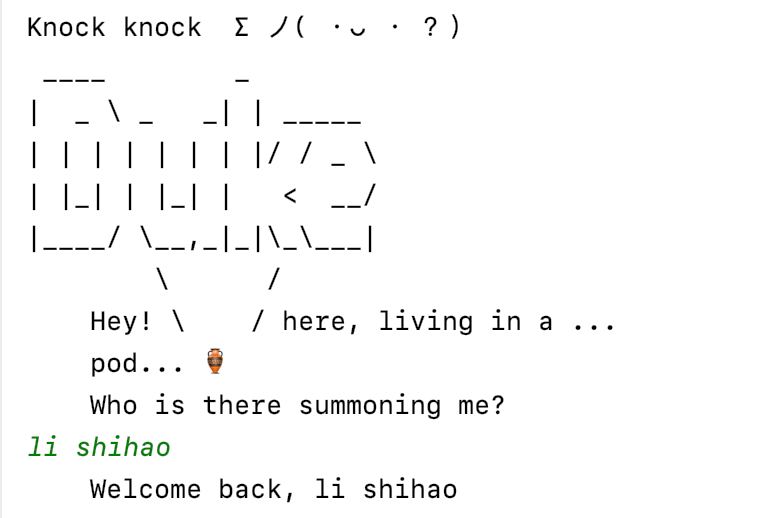
\includegraphics[height= 5.8cm]{startold.png}
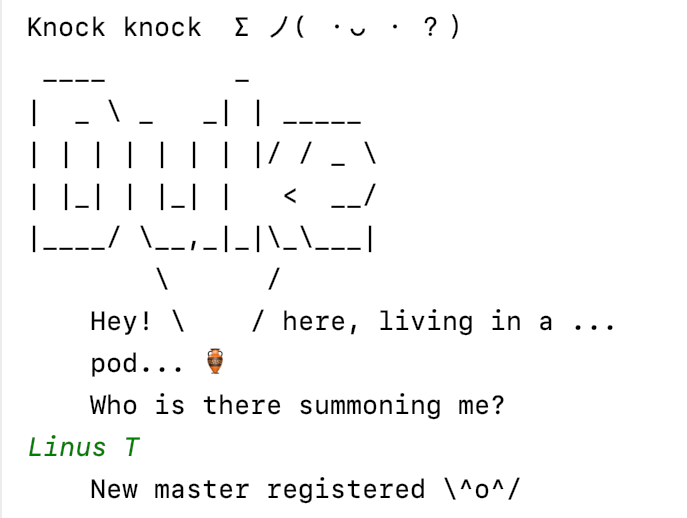
\includegraphics[height= 5.8cm]{startnew.png}
\caption{Screenshot - Start Greeting Page Existing/New User} 
\label{start}
\end{figure} 


\section* {Level-4 Describe the commands for adding different types of tasks} 
\begin{figure}[h]
\centering
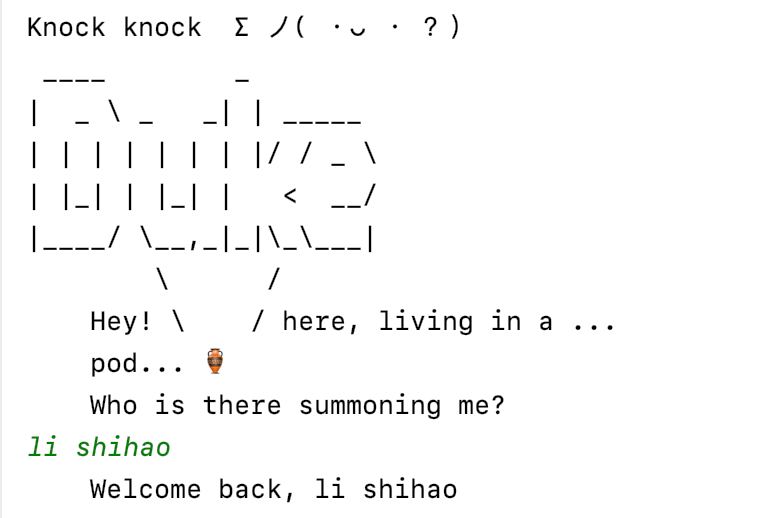
\includegraphics[height= 5.8cm]{startold.png}
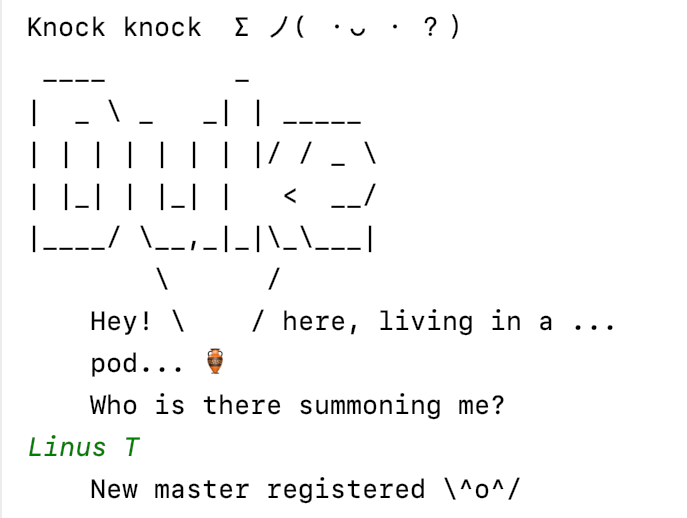
\includegraphics[height= 5.8cm]{startnew.png}
\caption{Screenshot - Start Greeting Page Existing/New User} 
\label{startold}
\end{figure} 



%\printbibliography

%\bibliography{assgn1}


\end{document}













